\documentclass[a4paper]{article}

\usepackage[english]{babel}
\usepackage[utf8]{inputenc}
\usepackage{amsmath}
\usepackage{graphicx}
\usepackage[colorinlistoftodos]{todonotes}
\usepackage{cite}
\usepackage{float}
\usepackage{algorithm}
\usepackage{algpseudocode}
\usepackage{amssymb}

\bibliographystyle{plain}
\title{Peer Grading}

\author{Mert Can ÇIKLA, Emre BEKTAŞ}

\date{\today}

\begin{document}
\maketitle
\abstract
Massive open-access online courses serve the purpose of providing free, high level education in
vast scales. Peer assessment is an important part of these courses where the number of peers can
scale up to tens of thousands. However peer assesment is still far perfect from getting on level with instructor grading. Bias of the peers and their accuracy in grading another peer are
matters that require work to make peer assessment more usable in practice. In the case where the assignments
are open to interpretation and can not be graded in an automated manner, various peer grading methods
are needed. In this study we delve into some highly popular peer grading methods. We identify and differentiate
them considering their way of approaching the problem. We experiment on various forms of synthetically generated data
in order to measure their performance in a simulated environment. We propose three ideas to improve accuracy and reduce error in peer grading.

\section{Introduction}
In recent years, massive open-access online courses (MOOCs) have gotten immensely popular and being free and requiring only an internet connection are the main reasons why. It allows people from all across the world to enroll and study at their own pace. Although this means online education can
be provided in huge scales, there is however a problem that arises if the students need to be examined. In a case where the exam can not be assessed by a computer whether it is due to its type ---such as an essay--- or the nature of the field of study. Most popular solution to this problem is
peer assesment where every peer grades certain amount of other peer's exams which in the end
will build up to be that peer's grade for that exam.
Peer grading is the most efficient way to evaluate when the peer count reaches thousands but it has it's flaws. Peers with no incentive to spend time on grading is a huge problem in peer assessment. Various studies \cite{Walsh14a,PiechHCDNK13,Alfaros13}have tried to incentivize this effort by giving a portion of the final grade to the grader depending on how accurately they have graded compared to others. Due to the vast scale of the peers and their different backgrounds, this does not always suffice to reduce error. It might be that one does not want to 
spend time on grading and grades randomly or one might not be knowledgeble about a certain
subject and may not grade others precisely. There are a lot more similar challenges to be
overcome in this case where you have next to no information about how skilled a peer 
is in evaluating so there are a lot of unknown variables in the equation.

In this study we identify the problem of peer grading and review the solution methods that have been
proposed and implemented in the literature. In the implementation details section we carefully explain
our methodology and our algorithms we use when testing on the current methods. In experiments section
we give detailed graphs of the experimentations we held and analyze the methods on various forms of 
synthetic data. Finally we identify some of the issues with peer grading and try to point out possible
improvements that are to be implemented and tested in the future.
\section{Literature Review}
	There have been various studies to increase the use of Peer Grading by reducing the error
 induced in evaluation. Walsh's \cite{Walsh14a} adapts PageRank ---the website ranking algorithm
   used by Google--- \cite{page1999pagerank} to peer grading. \textbf{PeerRank} method
constructs a matrix composed of grades and computes peer grades depending on their own grade and
their bias as a grader. The GeneralizedPeerRank adds the notion of reliability that couples
grader's accuracy in grading with their own grading to incentivize correct grading and reduce
error. Another method that incorporates bias and grader performance is \textbf{CrowdGrader}
    \cite{Alfaros13}. It combines the
grades provided by the students into a consensus grade for each submission students make by
utilizing an algorithm that relies on a reputation system. The algorithm computes a resulting
grade for each submission students make by weighing the students input grade by
their accuracy which are then used to update each students estimated accuracy of grading.This
algorithm seems to outperform median and average reliabilty
computation techniques but shows mixed results over real life data.
The authors also questioned whether it is best to use solely ranking or grading.

	Piech et al.\cite{PiechHCDNK13} defined 3 statistical models for peer grading. The first one
\textbf{PG1} attempts to detect grader's bias and compensate accordingly. Authors try to
make use of any possible coherence between a peer's performancwe on two different
assignments at different times with \textbf{PG2}. \textbf{PG3} relates a peer's evaluation
performance and grade like the method in \cite{Walsh14a}. They have experimented with these
methods on a dataset obtained from a sizeable MOOC and report significant improvements.

	Another approach used in the literature is to work on rankings instead of a cardinal grade.
This approach eases the load of students by asking for pairwise comparisons or a set of rankings 
but lacks in the value of information retrieved. The method in \cite{Shah13} compares ranking 
methods to those who only grade and show cases where making pairwise comparisons reduce error in 
comparison to cardinal evaluation. Their work extends the Bradley-Terry-Luce Model 
\cite{BT52,luce60} to peer grading and report ordinal evaluation to be more robust to lack of 
grader expertise.

The work of \cite{RamanJ14} tackles the Peer Grading as a rank aggregation and extends works of 
\cite{BT52,citeulike:7065887,PL,thurstone1927method}. They evaluated those methods on data 
gathered from a University course and show that Ordinal methods are in some cases superior to 
PG1 of \cite{PiechHCDNK13}.
\section{Implementation Details}
	We have prepared a Java program that enables us to run experiments with varying number of 
participants. In order to generate this synthetic we have used the following algorithm.\\
    
\begin{algorithm}
  \caption{Grade Assignment Algorithm}
  \label{alg:alg1}
  \begin{algorithmic}
    \State gen$(s)$	\Comment{$s$: size of class, $w$: workload}
    \State$S_i \gets G_{i+1} .. G_{i+5}$   \Comment{students $i+1 .. i+5$ grade student $i$} 
    \For{$i\gets 1, s$}
   		\State$rg_i\gets \mathcal{N}(70,30)$ \Comment{real grade of the student}
        \If{$rg_i < 0$}
           \State $g_i\gets 0$
        \ElsIf{$rg_i\ge 100$}
           \State $g_i\gets 100$
        \Else
            \State $g_i \gets rg_i$
        \EndIf
    \EndFor
  \end{algorithmic}
\end{algorithm}

\textbf{Algorithm 1} creates a classroom of $s$ students and assignes them $w$ graders and a
grade sampled from a normal distribution $\mathcal{N}$ with $\mu=70$ and $\sigma=30$. Also note that we have
also experimented with various other distributions.

\begin{algorithm}
\begin{algorithmic}
  \caption{Sum of Binomials Marking Model}
  \label{alg:alg2}
  
    \State review$(s)$	\Comment{$s$: size of class, $w$: workload}
    \ForAll{$G_{i,j}$} \Comment{$j$th grader of the student $i$}
   		\State$\alpha = \mathcal{B}(rg_i,rg_{G_{i,j}})$ \Comment{ $\mathcal{B}(n,p)$ n trials
        and p probability}
        \State$\beta = \mathcal{B}(100-rg_i,1-rg_{G_{i,j}})$
        \State$g_{i,j}= \alpha+\beta$;
    \EndFor
    
  \end{algorithmic}
\end{algorithm}
\ref{alg:alg2} was proposed by Walsh in \cite{Walsh14a} and models a very intuitive way of assigning grades. Aside from the $\alpha$ component which is straight-forward and represents a student grading correctly a question that is correct. The $\beta$ component of the mark is added by getting his wrong solution incorrectly
graded as correct. However an issue arrises with this model that, when a student with a real grader lower than 50 grades a similar grade student they grade themselves much higher than possibly anticipated. For instance, assume the grade of every student in the classroom is 20, this yields on average a marking of 80 $bin(20,0.2) = \alpha \approx 16 + bin(80,0.8) = \beta \approx 64$ even though one would expect an average grade of 20.
We have implemented \textbf{Algorithm 1} and \textbf{2} to measure performance of different peer
grading algorithms in the literature. The PeerRank and GeneralizedPeerRank methods
\cite{Walsh14a} were implemented by us. To measure the algorithm in \cite{Alfaros13} we used
their implementation. The ranking methods described in \cite{RamanJ14} were also measured using
the author's implementation after verification.\\

\clearpage
\section{Experiments}
Throughout the experiments PR refers to Peer Rank \cite{Walsh14a} and GPR refers to Generalized Peer Rank from the same 
paper. CG refers to CrowdGrader of \cite{Alfaros13}. MAL refers to Mallow's model originally proposed by Mallow \cite{citeulike:7065887} and adapted to peer assessment by \cite{RamanJ14}. MALS is the score-weighted Mallow's model and MALBC is Mallow's model with Borda count approximation also proposed by Raman and Joachims\cite{RamanJ14}. BT which stands for Bradley-Terry Model, THUR abbrevation of Thurstone model and PL the Plackett-Luce Model are also explained by Raman and Joachims in \cite{RamanJ14}. NCS is the PG1 model proposed by Piech et al. \cite{PiechHCDNK13} but with a maximum likelihood estimator instead of Gibbs Sampler.

Our first set of experiments figures 1 to 4 are based on the experiments conducted by Walsh in \cite{Walsh14a}. We have created a synthetic dataset using \ref{alg:alg1} and \ref{alg:alg2}. The dataset has 500 students with each student assigned to grade 5 other. Note that the original experiment by Walsh used 10 students all grading eachother, with that said our results verify those of Walsh in \cite{Walsh14a} and show almost exact results.
\begin{figure}[hb]
\centering
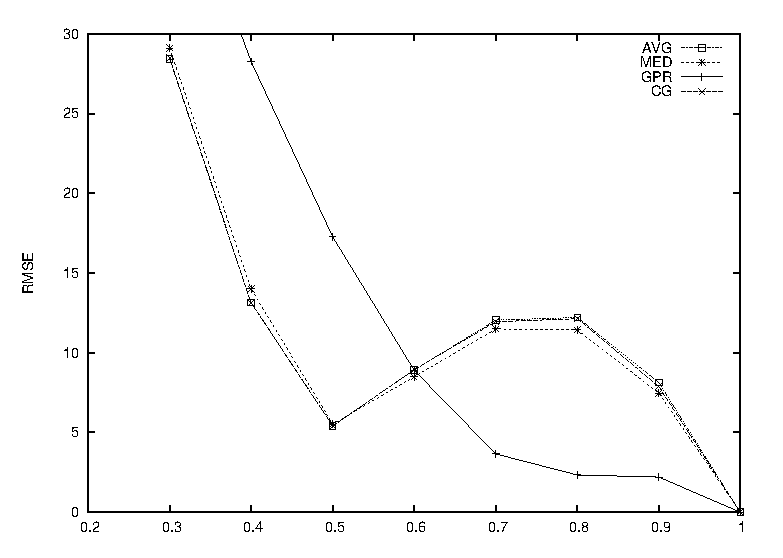
\includegraphics[width=1\textwidth]{figure01}
\caption{Binomial distribution with varying probability.}
\end{figure}

\newpage
\begin{figure}[H]
\centering
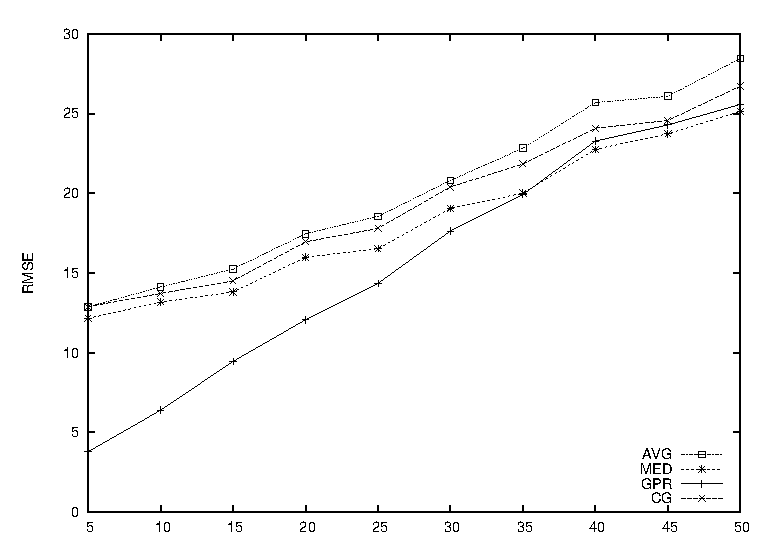
\includegraphics[width=1\textwidth]{figure02}
\caption{Normal distribution with increasing stdev.}
\end{figure}

\begin{figure}[H]
\centering
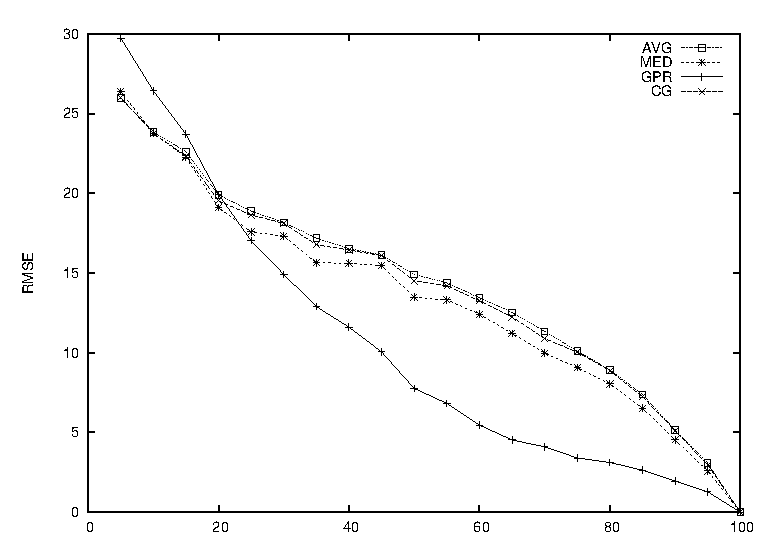
\includegraphics[width=1\textwidth]{figure03}
\caption{Uniform distribution with increasing lower bound.}
\end{figure}

\begin{figure}[H]
\centering
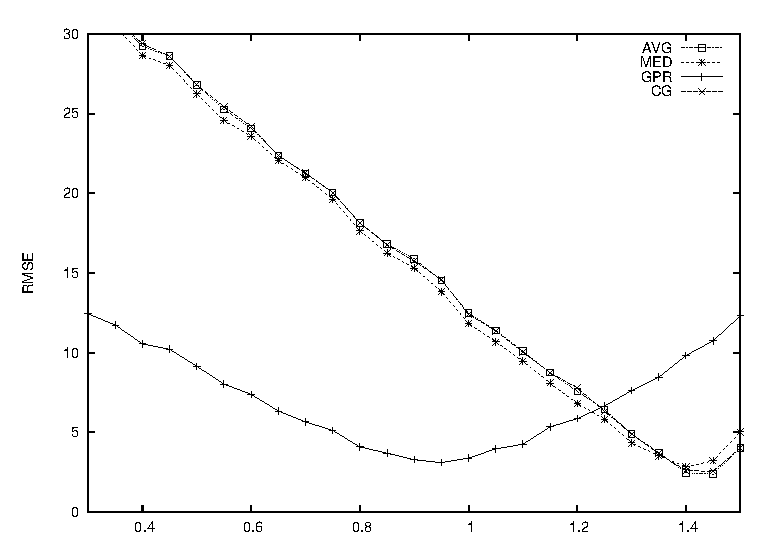
\includegraphics[width=1\textwidth]{figure04}
\caption{Normal distribution with varying grader bias.}
\end{figure}
\clearpage

In order to compare ordinal methods' performance with cardinals' we have conducted the following
experiments using grades coming from Binomial, Normal and Uniform distributions and we have
measured their Kendall-$\tau$ distances. Kendall-$\tau$ is the total miss ordering of a method
compared to the realgrade(instructor) ordering.\\

\begin{figure}[hb]
\centering
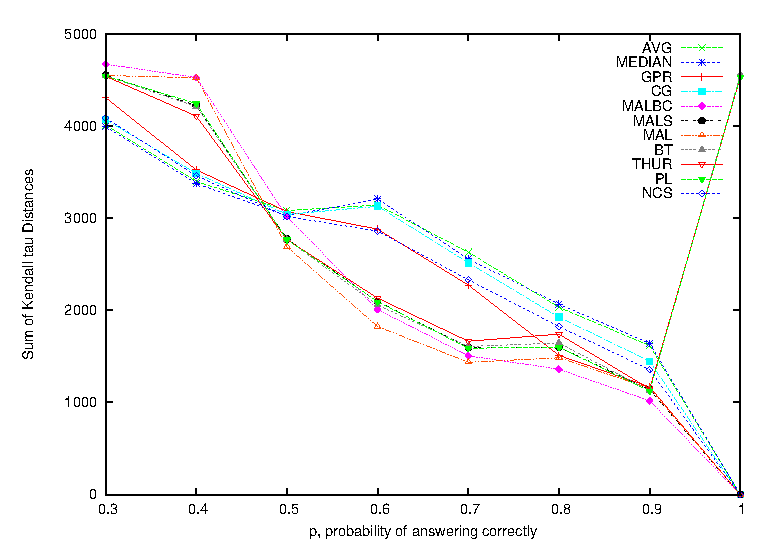
\includegraphics[width=1\textwidth]{figure1}
\caption{Binomial distribution with varying probability.}
\end{figure}

\newpage
\begin{figure}[H]
\centering
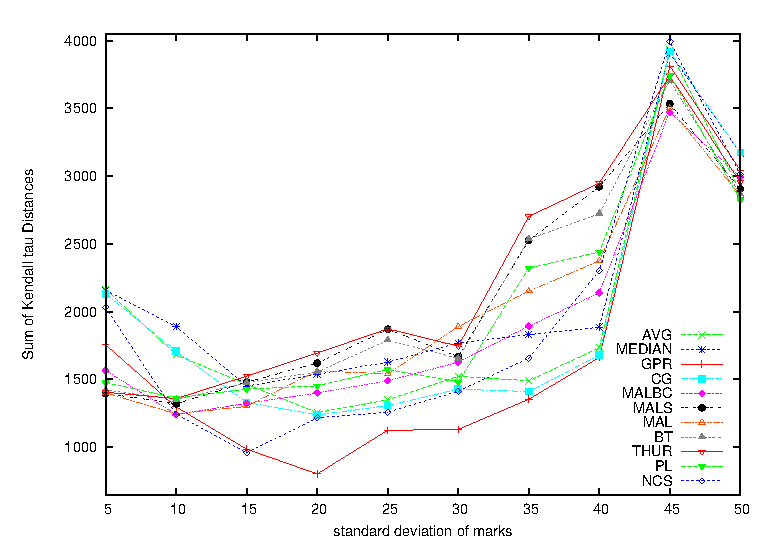
\includegraphics[width=1\textwidth]{figure2}
\caption{Normal distribution with increasing stdev.}
\end{figure}

\begin{figure}[H]
\centering
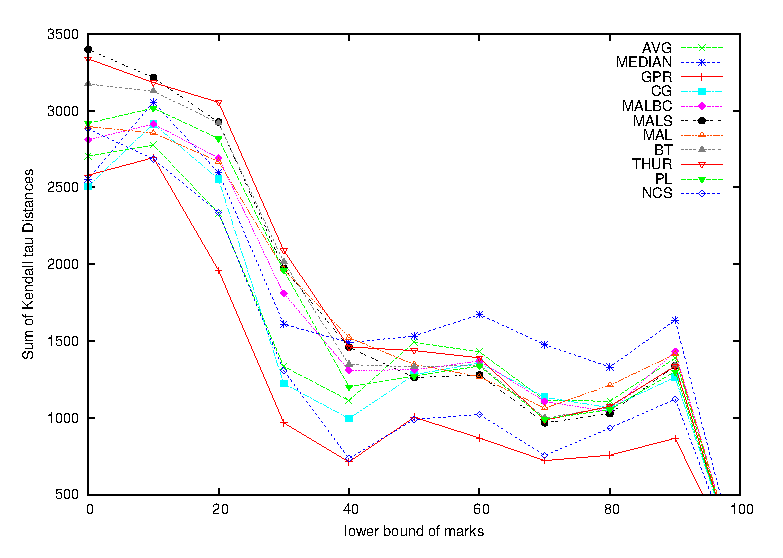
\includegraphics[width=1\textwidth]{figure3}
\caption{Uniform distribution with increasing lower bound.}
\end{figure}
\clearpage
 
The experiments show the Generalized PeerRank method proposed by \cite{Walsh14a} outperforms
others when the grades are Normally or Uniformly distributed. However the method seems to be
average when the grades are Binomial. 

\section{Future Work}
First possible improvement we have theorised is to improve the Generalized PeerRank by looking
at the cause of sub-par performance when the grades are Binomially distributed as it is odd for
the results to be vastly different although the Binomial and Normal cases map a very similar
distribution of grades overall.

Our second idea for improvement is to gather new information about students by splitting the
exam into parts according to a rubric or simply grading each question seperately. Consider the
case where a student has gotten a full-mark from the first question but zero marks from the
second. In this case the student can be a much more effective as a grader if we can assign the
student to only grade the first question for this exam instead of the exam as a whole. This
methodology is not limited to exams that can be divided into questions. Any exam with a rubric
is an applicable case since for example the grammar used in an English essay can be graded by
a grader with grammar expertise and another can grade its cohesion.

Lastly there is a decent chance of extracting valuable information by finding a coherence between 
a peer's performance on different times. The likely coherence and identification of this should 
help better estimate a grader's reliability.

\section{Conclusion}
MOOCs are essential to take the education to the next era and Peer Grading has a crucial part in
this. However Peer Grading methods still have a long way to go to reduce the error induced due to malicious grading or lack of grading performance.

We have experimented using synthetically generated data and distinguished Generalized PeerRank method proposed by \cite{Walsh14a} to be the method with the least error induced and we are planning to work on ways of improving this particular method.

We also propose an idea that has great potential to improve grading performance by assigning graders things that they are relatively more knowledged about.
\clearpage
\bibliography{report3}{}
\end{document}